\documentclass[12pt,a4paper]{article}
\usepackage[top=1.5cm, bottom=1.5cm, left=2.0cm, right=1.5cm] {geometry}
\usepackage{amsmath,amssymb}
\usepackage{tkz-euclide}
\usepackage{tikz,tkz-tab}
\usepackage[loigiai]{ex_test}
\def\colorEX{\color{purple}}
\renewtheorem{ex}{\color{violet}Câu}
\begin{document}
	\begin{center}
		\textbf{SOẠN THẢO CÂU TRẮC NGHIỆM }
	\end{center}
	\Opensolutionfile{ans}[ans/ans192]
	%% LaTeX2e file `hamso.tex'
\documentclass[12pt,a4paper]{article}
\usepackage[top=1.5cm, bottom=1.5cm, left=2.0cm, right=1.5cm] {geometry}
\usepackage{amsmath,amssymb}
\usepackage{tkz-euclide}
\usepackage{tikz,tkz-tab}
\usepackage[loigiai]{ex_test}
\def\colorEX{\color{purple}}
\begin{document}
\begin{ex}%[0D2B2-3]
Đường thẳng nào dưới đây là tiệm cận ngang của đồ thị hàm số $y=\dfrac{-3x+1}{x+2}?$
\choice
{$x=-3$}
{\True $y=-3$}
{$x=-2$}
{$y=\dfrac{1}{2}$}
\end{ex}

\begin{ex}%[0D2B2-1]
Bảng biến thiên ở hình bên là của một trong bốn hàm số được liệt kê dưới đây.
\begin{center}
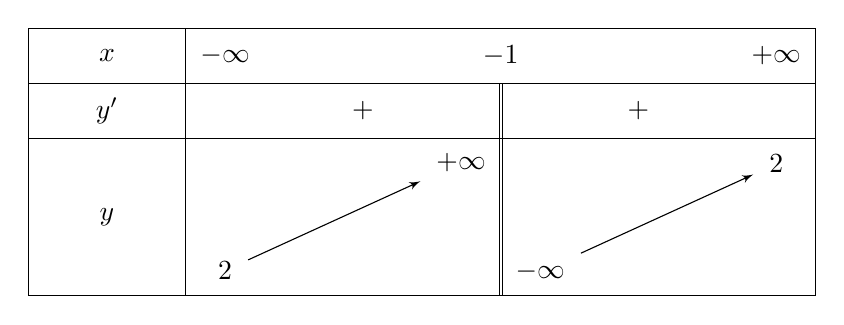
\begin{tikzpicture}
\tkzTabInit[espcl=3.5]
{$x$ /.7, $y'$ /.7,$y$ /2}{$-\infty$ , $-1$ , $+\infty$}
\tkzTabLine{ ,+,d,+, }
\tkzTabVar{-/$2$ ,+D- / $+\infty$/$-\infty$, +/ $2$}
\end{tikzpicture}
\end{center} Hãy tìm hàm số đó.
\choice{$y=\dfrac{-x+1}{x-2}$}{\True $y=\dfrac{2x-3}{x+1}$}{$y=\dfrac{-2x-3}{x+1}$}{$y=\dfrac{2x+3}{x-1}$}
\end{ex}
\begin{ex}%[0D2K2-1]
Cho hàm số $y=\dfrac{1}{3}x^3-\dfrac{1}{2}x^2-12x-1.$ Mệnh đề nào sau đây là đúng?
\choice
{Hàm số đồng biến trên khoảng $(-\infty;4)$}
{\True Hàm số đồng biến trên khoảng $(4;+\infty)$}
{Hàm số nghịch biến trên khoảng $(-3;+\infty)$}
{Hàm số đồng biến trên khoảng $(-3;4)$}
\end{ex}
\begin{ex}%[0D2K3-3]
Trong các hàm số sau, hàm số nào có hai điểm cực đại và một điểm cực tiểu?
\choice{$y=x^4-x^2+3$}{\True $y=-x^4+x^2+3$}{$y=x^4+x^2+3$}{$y=-x^4-x^2+3$}
\end{ex}
\begin{ex}%[0D2G3-3]
Tìm giá trị cực tiểu của hàm số $y=\dfrac{x^2+3}{x+1}.$
\choice{$-6$}{\True $2$}{$1$}{$-3$}
\end{ex}
\begin{ex}%[0D2K3-4]
Cho hàm số $y=x^4-2mx^2+1-m.$ Tìm tất cả các giá trị thực của $m$ để đồ thị hàm số có ba điểm cực trị tạo thành một tam giác nhận gốc tọa độ $O$ làm trực tâm.
\choice{$m=0$}{\True $m=1$}{$m=-1$}{$m=2$}
\end{ex}
\begin{ex}%[0D2K3-3]
Tìm tất cả các đường tiệm cận ngang của đồ thị hàm số $y=\dfrac{2x+1+\sqrt{x^2+1}}{x-3}.$
\choice{$y=3$}{\True $y=3$ và $y=1$}{$y=1$}{$y=2$}
\end{ex}
\begin{ex}%[0D2K2-4]
Biết đường thẳng $y=3x+4$ cắt đồ thị hàm số $y=\dfrac{4x+2}{x-1}$ tại hai điểm phân biệt có tung độ là $y_1$ và $y_2$. Tính $y_1+y_2.$
\choice{$y_1+y_2=1$}{\True $y_1+y_2=11$}{$y_1+y_2=9$}{$y_1+y_2=10$}
\end{ex}
\begin{ex}%[0D2B3-1]
Cho hàm số $y=f(x)$ xác định trên $\mathbb{R}\setminus \{1\},$ liên tục trên từng khoảng xác định, và có bảng biến thiên như dưới đây.
\begin{center}
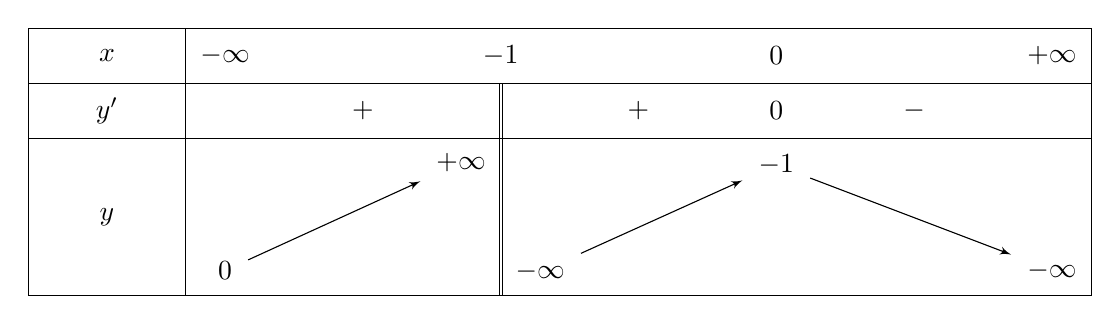
\begin{tikzpicture}
\tkzTabInit[espcl=3.5]
{$x$ /.7, $y'$ /.7,$y$ /2}{$-\infty$ , $-1$ , $0$ , $+\infty$}
\tkzTabLine{ ,+,d,+,0,-, }
\tkzTabVar{-/$0$ ,+D- / $+\infty$/$-\infty$, +/ $-1$,-/$-\infty$}
\end{tikzpicture}
\end{center}
Tìm tập hợp tất cả các giá trị thực của $m$ để phương trình $f(x)=m$ có nghiệm thực duy nhất.
\choice{$[0;+\infty)\cup \{-1\}$}{\True $(0;+\infty)\cup \{-1\}$}{$(0;+\infty)$}{$[0;+\infty)$}
\end{ex}
\begin{ex}%[0D2G3-5]
Cho hàm số $y=x^3-6x^2+9x+m$ ($m$ là tham số thực) có đồ thị $(C)$. Giả sử $(C)$ cắt trục hoành tại 3 điểm phân biệt có hoành độ $x_1,x_2,x_3$ (với $x_1<x_2<x_3$). Khẳng định nào sau đây đúng?
\choice{$1<x_1<x_2<3<x_3<4$}{\True $0<x_1<1<x_2<3<x_3<4$}{$x_1<0<1<x_2<3<x_3<4$}{$1<x_1<3<x_2<4<x_3$}
\loigiai{
\textbf{Cách 1:} Thay $m$ bằng một giá trị âm bất kì và casio.\\
\textbf{Cách 2:} Dễ có $m<0$
}
\end{ex}
\begin{ex}%[0D2G3-3]
\ \newline
\begin{minipage}[h]{12cm}
Đồ thị hàm số $y=ax^4+bx^2+c$ cắt trục hoành tại bốn điểm phân biệt $A,B,C,D$ như hình vẽ bên. Biết rằng ${\displaystyle AB=BC=CD},$ mệnh đề nào sau đây đúng?
\end{minipage}\hspace{1cm}
\begin{minipage}[h]{5cm}
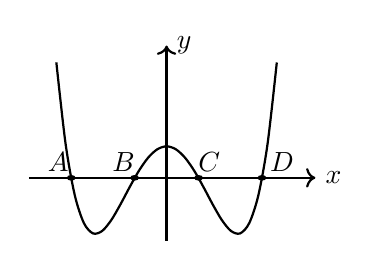
\begin{tikzpicture}[xscale=.7, yscale=.4]
\draw[->][thick] (-2.5,0) -- (2.7,0) node[right] {$x$};
\draw[->][thick] (0,-2) -- (0,4.2) node[right] {$y$};
\draw[smooth,domain=-2:2][thick] plot(\x,{(\x)^4-10/3*(\x)^2+1}) ;
\draw(-1.6,0.5) node[left]{$A$};
\draw(1.7,0.5) node[right]{$D$};
\draw(-0.4,0.5) node[left]{$B$};
\draw(0.4,0.5) node[right]{$C$};
\filldraw[black](-1.73,0) circle(2pt);
\filldraw[black](-.58,0) circle(2pt);
\filldraw[black](1.73,0) circle(2pt);
\filldraw[black](.58,0) circle(2pt);
\end{tikzpicture}
\end{minipage}
\choice{$a>0,b>0,c>0,9b^2=100ac$}{\True $a>0,b<0,c>0,9b^2=100ac$}{$a>0,b>0,c>0,100b^2=9ac$}{$a>0,b<0,c>0,100b^2=9ac$}
\loigiai{
Từ hình dạng đồ thị, ta suy ra $a>0, b<0, c>0$ (nhánh vô cực, 3 cực trị, cắt trục tung tại điểm có tung độ dương).\\
Phương trình $ax^4=bx^2+c=0$ có bốn nghiệm lập thành cấp số cộng, tương đương phương trình $at^2+b^t+c$ có hai nghiệm $0<t_1<t_2$, với $\sqrt{t_2}-\sqrt{t_1}=\sqrt{t_1}-\left(-\sqrt{t_1}\right)\Rightarrow t_2=9t_1$.\\
Lại có $t_1+t_2=-\dfrac{b}{a}\Rightarrow t_1=-\dfrac{b}{10a}$ và $t_2=-\dfrac{9b}{10a}$.\\
Hơn nữa $t_1.t_2=\dfrac{c}{a}\Rightarrow \dfrac{9b^2}{100a^2}=\dfrac{c}{a}\Rightarrow 9n^2=100ac$.\\
\textbf{Chú ý:} Cũng có thể lấy $t_1=1, t_2=9$ ta được phương trình $x^4-10x^2+9=0$.
}
\end{ex}

\end{document}
	\Closesolutionfile{ans}
	\begin{center}
		\textbf{ĐÁP ÁN CÂU TRẮC NGHIỆM}
	\end{center}
	\begin{multicols}{10}
		\begin{Solution}{1}
B
\end{Solution}
\begin{Solution}{2}
B
\end{Solution}
\begin{Solution}{3}
B
\end{Solution}
\begin{Solution}{4}
B
\end{Solution}
\begin{Solution}{5}
B
\end{Solution}
\begin{Solution}{6}
B
\end{Solution}
\begin{Solution}{7}
B
\end{Solution}
\begin{Solution}{8}
B
\end{Solution}
\begin{Solution}{9}
B
\end{Solution}
\begin{Solution}{10}
B
\end{Solution}
\begin{Solution}{11}
B
\end{Solution}

	\end{multicols}
\end{document}